% !TeX encoding = UTF-8
\chapter{Task 4: Machine Learning Classifiers}\label{chap:task4_ml}

\section{Setup}\label{sec:ml-setup}

We train Logistic Regression (LR, \texttt{max\_iter=5000}) and a Decision Tree (DT, \texttt{random\_state=42}, unpruned) with scikit-learn~\cite{pedregosa2011sklearn}. Each is trained in two variants, default and \texttt{class\_weight="balanced"}, and for two targets: binary (BENIGN vs.\ ATTACK) and multiclass (four labels). This gives eight models. Every model is one scikit-learn \texttt{Pipeline}: \texttt{MinMaxScaler(clip=True)}, \texttt{SelectKBest(chi2, k=20)} and the classifier (Listing~\ref{lst:pipe}). Scaler and selector are fitted on the training split only (114,925 flows). All models are evaluated on the held-out test split of 49,254 flows, of which 643 are attacks. The selected features of every saved pipeline equal the Task 3 lists exactly, and all four LR models converged well below the iteration limit. Inference time is the median of five timed \texttt{predict} calls on the whole test split after one warm-up call, scaled to 1,000 flows. Because of the imbalance, we report precision, recall, F1, macro-F1 and confusion matrices, not accuracy alone.

\lstinputlisting[style=py,float=htbp,linerange={21-27,29-37},caption={\texttt{build\_pipeline()} and \texttt{make\_classifier()} in \texttt{src/lab2ids/models.py}},label={lst:pipe}]{../src/lab2ids/models.py}

\section{Binary Results}\label{sec:ml-binary}

Table~\ref{tab:t4binary} shows the binary results. The default Decision Tree is the best model: it detects all 643 attacks (recall 1.0000) with 18 false positives and an attack F1 of 0.9862. Its balanced variant is almost identical. Logistic Regression is clearly worse. The default LR misses 94 attacks (recall 0.8538). With \texttt{class\_weight="balanced"}, LR reaches a recall of 0.9907 but at a precision of only 0.2349, with 2,075 false alarms, ten times more than the default (201). Figure~\ref{fig:cm} (a) and (b) show the confusion matrices of the two models.

\begin{table}[ht]
	\centering\small
	\resizebox{\linewidth}{!}{% AUTO-GENERATED by scripts/make_report_tables.py from outputs/task4/comparison.csv, outputs/task4/metrics.json -- do not edit
\begin{tabular}{lrrrrrrrrr}
\toprule
Model & Acc. & Macro-F1 & Prec. & Rec. & F1 & FP & FN & Fit (s) & Inf. (ms/1k) \\
\midrule
LR default & 0.9940 & 0.8926 & 0.7320 & 0.8538 & 0.7882 & 201 & 94 & 5.74 & 0.708 \\
LR balanced & 0.9577 & 0.6789 & 0.2349 & 0.9907 & 0.3797 & 2\,075 & 6 & 23.26 & 0.672 \\
\textbf{DT default} & \textbf{0.9996} & \textbf{0.9930} & \textbf{0.9728} & \textbf{1.0000} & \textbf{0.9862} & \textbf{18} & \textbf{0} & \textbf{0.36} & \textbf{0.667} \\
DT balanced & 0.9996 & 0.9925 & 0.9815 & 0.9891 & 0.9853 & 12 & 7 & 0.35 & 0.683 \\
\bottomrule
\end{tabular}
}
	\caption{Binary results on the test split (Prec., Rec., F1 refer to the attack class; FP/FN are false positives and false negatives). Best model in bold.}
	\label{tab:t4binary}
\end{table}

\section{Multiclass Results}\label{sec:ml-multi}

Table~\ref{tab:t4multi} shows the multiclass results. The default Decision Tree again leads with a macro-F1 of 0.7290. The default Logistic Regression reaches an accuracy of 98.54\,\% but detects \emph{no} attack at all (F1 of 0.0000 for all three attack classes, macro-F1 0.2482): it predicts almost everything as BENIGN (Figure~\ref{fig:cm} (d)). This is the accuracy paradox, since 98.7\,\% of the data is benign anyway. Class weighting raises the LR macro-F1 only to 0.3191 and lowers the DT macro-F1 to 0.5642. Within the DT, Brute Force and XSS are frequently confused (Figure~\ref{fig:cm} (c)): 103 Brute Force flows are predicted as XSS and 97 XSS flows as Brute Force. Both attacks are automated HTTP requests from the same client to the same web server, and flow statistics cannot see the payload, which is the only thing that really differs. SQL injection reaches an F1 of 0.9091, but with only 6 test flows (5 detected) this number is statistically weak: one flow more or less changes it by about 0.1.

\begin{table}[ht]
	\centering\small
	\resizebox{\linewidth}{!}{% AUTO-GENERATED by scripts/make_report_tables.py from outputs/task4/comparison.csv -- do not edit
\begin{tabular}{lrrrrrrrr}
\toprule
Model & Acc. & Macro-F1 & BENIGN & Brute Force & XSS & SQLi & Fit (s) & Inf. (ms/1k) \\
\midrule
LR default & 0.9854 & 0.2482 & 0.9926 & 0.0000 & 0.0000 & 0.0000 & 11.67 & 0.688 \\
LR balanced & 0.9321 & 0.3191 & 0.9689 & 0.0781 & 0.2233 & 0.0061 & 26.40 & 0.835 \\
DT default & 0.9923 & 0.7290 & 0.9982 & 0.6126 & 0.3960 & 0.9091 & 0.73 & 0.701 \\
DT balanced & 0.9913 & 0.5642 & 0.9977 & 0.5827 & 0.3762 & 0.3000 & 0.77 & 0.675 \\
\bottomrule
\end{tabular}
}
	\caption{Multiclass results on the test split. The columns BENIGN to SQLi are per-class F1 scores.}
	\label{tab:t4multi}
\end{table}

\begin{figure}[ht]
	\centering
	\begin{subfigure}[t]{0.48\linewidth}
		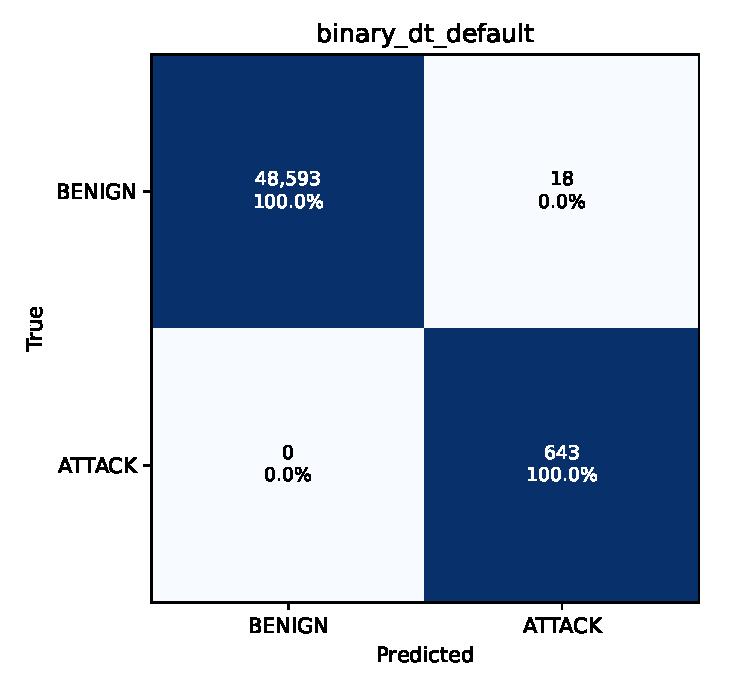
\includegraphics[width=\linewidth]{cm_binary_dt_default.pdf}
		\caption{Decision Tree (binary): all 643 attacks detected, 18 false positives.}
	\end{subfigure}\hfill
	\begin{subfigure}[t]{0.48\linewidth}
		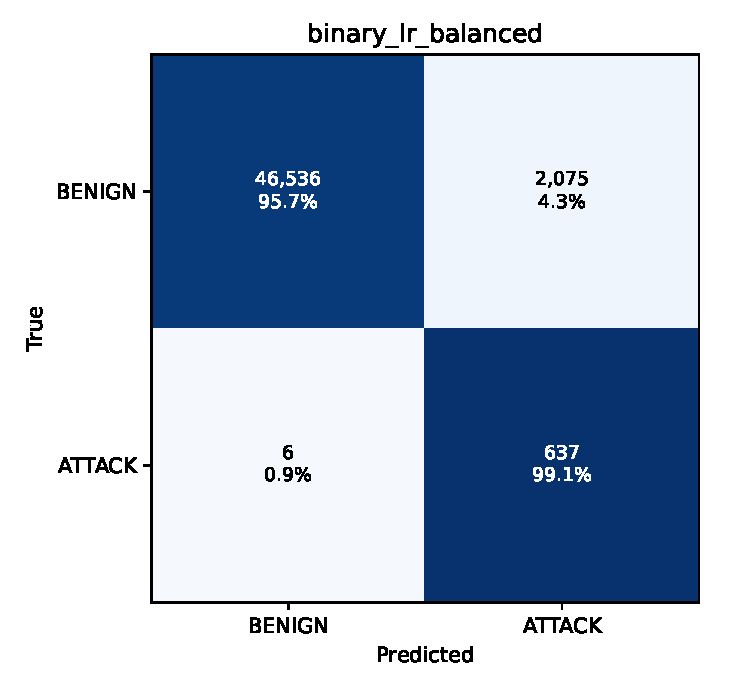
\includegraphics[width=\linewidth]{cm_binary_lr_balanced.pdf}
		\caption{Balanced Logistic Regression: 99\,\% attack recall at the cost of 2,075 false alarms.}
	\end{subfigure}\\[2pt]
	\begin{subfigure}[t]{0.48\linewidth}
		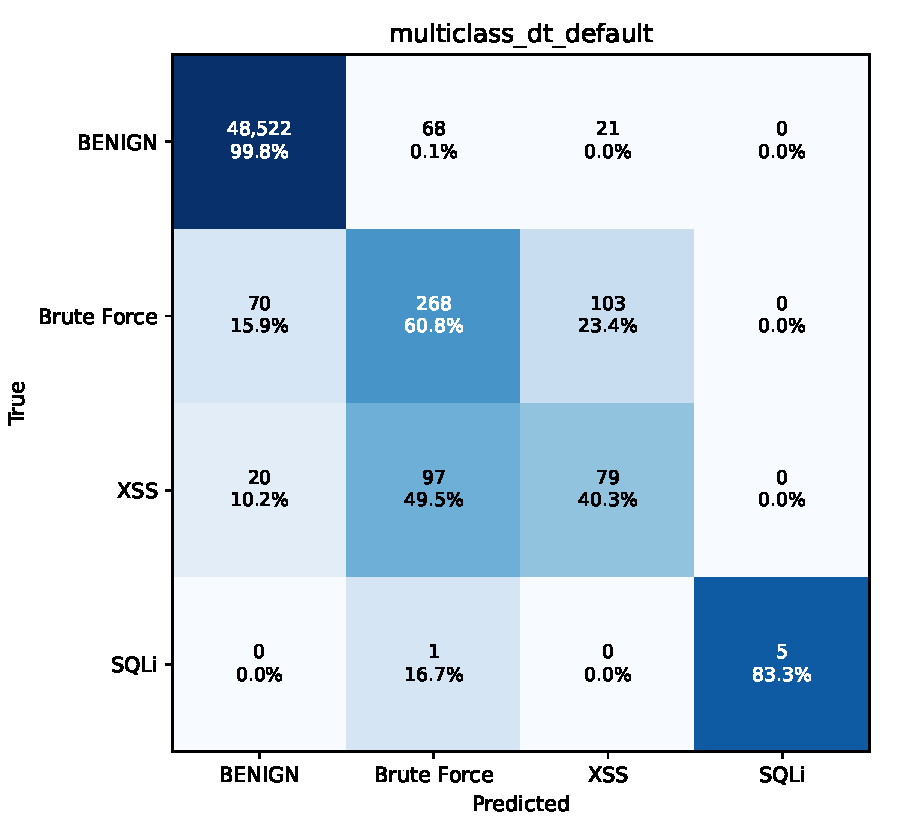
\includegraphics[width=\linewidth]{cm_multiclass_dt_default.pdf}
		\caption{Decision Tree (4 classes): Brute Force and XSS are frequently confused.}
	\end{subfigure}\hfill
	\begin{subfigure}[t]{0.48\linewidth}
		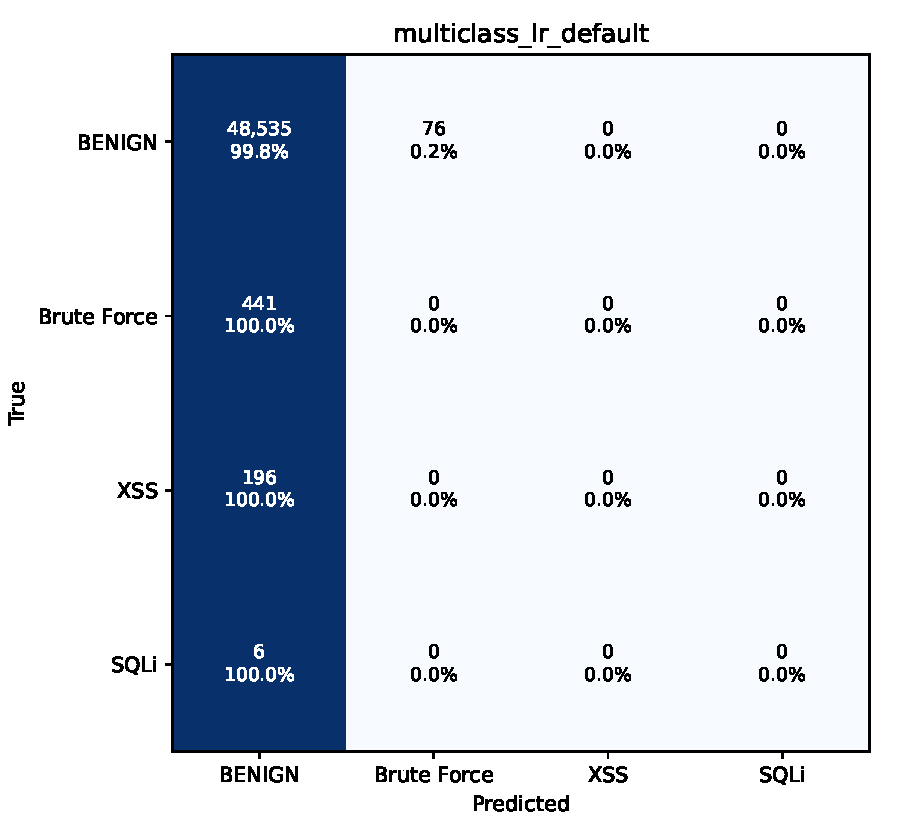
\includegraphics[width=\linewidth]{cm_multiclass_lr_default.pdf}
		\caption{Logistic Regression (4 classes) predicts almost everything as BENIGN: 98.5\,\% accuracy, 0 attacks detected.}
	\end{subfigure}
	\caption{Confusion matrices of four key models (test split).}
	\label{fig:cm}
\end{figure}

\begin{figure}[ht]
	\centering
	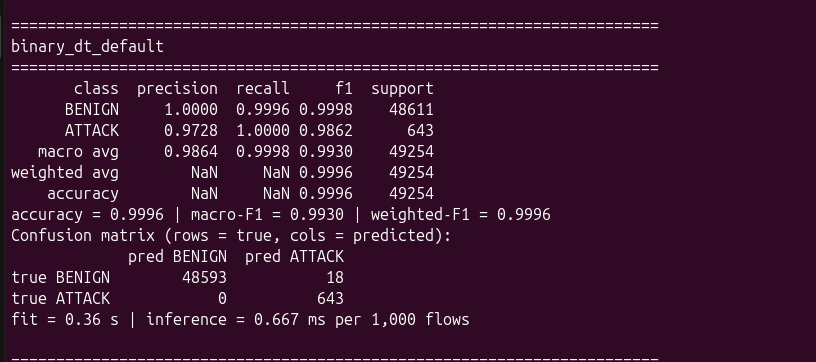
\includegraphics[width=0.8\linewidth]{SS3.png}
	\caption{Console output of the training script for the chosen model, the default Decision Tree (binary).}
	\label{fig:ss3}
\end{figure}

\section{Interpretation}\label{sec:ml-interp}

The Decision Tree beats Logistic Regression on both targets: attack F1 of 0.986 against at best 0.788, and multiclass macro-F1 of 0.729 against 0.319. Attacks are characterized by specific value ranges of a few features (small TCP windows, port 80, flag counts), which a tree isolates with axis-aligned thresholds. LR draws a single linear boundary through heavy-tailed, min-max-compressed features and cannot. Class weighting is a trade-off, not a fix: for LR it buys recall at the price of precision, and for the DT it hardly changes the binary result and hurts the multiclass result. The binary Decision Tree (default) is the model we use in the real-time part.

\FloatBarrier
